% Options for packages loaded elsewhere
\PassOptionsToPackage{unicode}{hyperref}
\PassOptionsToPackage{hyphens}{url}
\PassOptionsToPackage{dvipsnames,svgnames,x11names}{xcolor}
%
\documentclass[
]{article}
\usepackage{amsmath,amssymb}
\usepackage{iftex}
\ifPDFTeX
  \usepackage[T1]{fontenc}
  \usepackage[utf8]{inputenc}
  \usepackage{textcomp} % provide euro and other symbols
\else % if luatex or xetex
  \usepackage{unicode-math} % this also loads fontspec
  \defaultfontfeatures{Scale=MatchLowercase}
  \defaultfontfeatures[\rmfamily]{Ligatures=TeX,Scale=1}
\fi
\usepackage{lmodern}
\ifPDFTeX\else
  % xetex/luatex font selection
\fi
% Use upquote if available, for straight quotes in verbatim environments
\IfFileExists{upquote.sty}{\usepackage{upquote}}{}
\IfFileExists{microtype.sty}{% use microtype if available
  \usepackage[]{microtype}
  \UseMicrotypeSet[protrusion]{basicmath} % disable protrusion for tt fonts
}{}
\makeatletter
\@ifundefined{KOMAClassName}{% if non-KOMA class
  \IfFileExists{parskip.sty}{%
    \usepackage{parskip}
  }{% else
    \setlength{\parindent}{0pt}
    \setlength{\parskip}{6pt plus 2pt minus 1pt}}
}{% if KOMA class
  \KOMAoptions{parskip=half}}
\makeatother
\usepackage{xcolor}
\usepackage[margin=1in]{geometry}
\usepackage{longtable,booktabs,array}
\usepackage{calc} % for calculating minipage widths
% Correct order of tables after \paragraph or \subparagraph
\usepackage{etoolbox}
\makeatletter
\patchcmd\longtable{\par}{\if@noskipsec\mbox{}\fi\par}{}{}
\makeatother
% Allow footnotes in longtable head/foot
\IfFileExists{footnotehyper.sty}{\usepackage{footnotehyper}}{\usepackage{footnote}}
\makesavenoteenv{longtable}
\usepackage{graphicx}
\makeatletter
\def\maxwidth{\ifdim\Gin@nat@width>\linewidth\linewidth\else\Gin@nat@width\fi}
\def\maxheight{\ifdim\Gin@nat@height>\textheight\textheight\else\Gin@nat@height\fi}
\makeatother
% Scale images if necessary, so that they will not overflow the page
% margins by default, and it is still possible to overwrite the defaults
% using explicit options in \includegraphics[width, height, ...]{}
\setkeys{Gin}{width=\maxwidth,height=\maxheight,keepaspectratio}
% Set default figure placement to htbp
\makeatletter
\def\fps@figure{htbp}
\makeatother
\setlength{\emergencystretch}{3em} % prevent overfull lines
\providecommand{\tightlist}{%
  \setlength{\itemsep}{0pt}\setlength{\parskip}{0pt}}
\setcounter{secnumdepth}{5}
\usepackage[french]{babel} \usepackage{amsmath} \usepackage{geometry} \usepackage{fontspec} \usepackage{pdfpages} \usepackage{graphicx} \usepackage{amsmath} \usepackage{atbegshi} \usepackage{fancyhdr} \usepackage{tocloft} \usepackage{tcolorbox} \usepackage{xcolor} \definecolor{bleu}{RGB}{0,0,255} \usepackage{everypage} \pagestyle{fancy} \definecolor{mybrown}{RGB}{139,69,19} \fancyhead[R]{}
\ifLuaTeX
  \usepackage{selnolig}  % disable illegal ligatures
\fi
\usepackage{bookmark}
\IfFileExists{xurl.sty}{\usepackage{xurl}}{} % add URL line breaks if available
\urlstyle{same}
\hypersetup{
  colorlinks=true,
  linkcolor={Maroon},
  filecolor={Maroon},
  citecolor={Blue},
  urlcolor={blue},
  pdfcreator={LaTeX via pandoc}}

\author{}
\date{\vspace{-2.5em}}

\begin{document}

\setcounter{tocdepth}{5}                
\renewcommand\contentsname{\begin{center}\textcolor{brown}{Sommaire}\end{center}}

\AtBeginShipout{
  \ifnum\value{page}=1\thispagestyle{empty}\fi}

\pagestyle{fancy}
\fancyhf{}
\renewcommand{\headrulewidth}{0.4pt}
\renewcommand{\footrulewidth}{0.4pt}
\fancyhead[L]{Elèves Ingénieurs}
\fancyhead[R]{\textcolor{brown}{@Alex, Ali, Richard \& Toussaint}}
\fancyfoot[C]{\thepage}
\fancyfoot[L]{Mars 2025}
\fancyfoot[R]{Projet Statistique}

\AddEverypageHook{
  \ifnum\value{page}>1 
    \fancyhead[L]{Elèves Ingénieurs}
    \fancyhead[R]{\textcolor{brown}{@Alex, Ali, Richard \& Toussaint}}
    \fancyfoot[C]{\thepage}
    \fancyfoot[L]{Mars 2025}
    \fancyfoot[R]{Projet Statistique}
  \else
    \fancyhead[L]{} 
    \fancyhead[R]{}
    \fancyfoot[C]{}
    \fancyfoot[R]{}
  \fi
}

\tableofcontents

\newpage

\renewcommand\listtablename{\begin{center}\textcolor{brown}{Liste des Tableaux}\end{center}}
\renewcommand\listfigurename{\begin{center}\textcolor{brown}{Liste des Figures}\end{center}} 

\setlength{\cftfignumwidth}{3em}
\setlength{\cfttabnumwidth}{3em}

\listoftables

\newpage

\listoffigures

\newpage

\begin{center}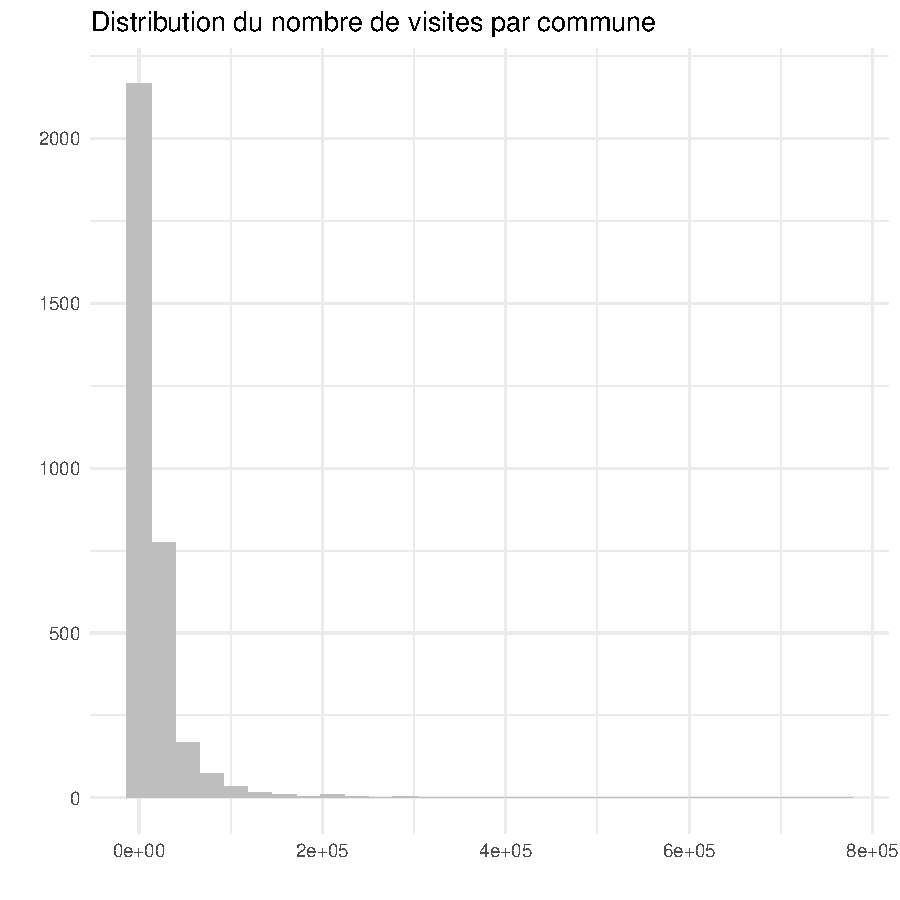
\includegraphics{Rapport_Projet_Stat_Ensai_files/figure-latex/unnamed-chunk-1-1} \end{center}

\section{Introduction}\label{introduction}

\section{Présentation du contexte}\label{pruxe9sentation-du-contexte}

\subsection{Intérêt de l'étude}\label{intuxe9ruxeat-de-luxe9tude}

\subsection{Cadre conceptuel de
l'étude}\label{cadre-conceptuel-de-luxe9tude}

\subsection{Présentation des
données}\label{pruxe9sentation-des-donnuxe9es}

\section{Méthodologie}\label{muxe9thodologie}

\section{Analyse des résultats}\label{analyse-des-ruxe9sultats}

\subsection{Analyse descriptive}\label{analyse-descriptive}

Dans cette partie, nous allons réaliser quelques statistiques
descriptives sur nos données.

\subsubsection{Analyse univariée}\label{analyse-univariuxe9e}

\subsubsection{Analyse bivariée}\label{analyse-bivariuxe9e}

Nous allons ici, voir s'il y a un lien à priori entre le taux de
consultation et certaines de nos variables explicatives. Ainsi, nous
avons d'abord réalisé une analyse descriptive bivariée puis nous avons
calculé la corrélation de Pearson pour évaluer le lien linéaire entre le
taux de consulation et des variables telles que la population totale, la
part des personnes agées (75 ans et plus), la part de quelques CSP
(ouvriers et retraités).

\paragraph{Taux de consultation et population
totale}\label{taux-de-consultation-et-population-totale}

\begin{verbatim}
## # A tibble: 3 x 2
##   taille_commune consultations_moyennes
##            <int>                  <dbl>
## 1              1                   1.38
## 2              2                   1.46
## 3              3                   1.53
\end{verbatim}

En divisant les communes en trois groupes égaux (ou presque égaux) en
fonction de la population totale, il ressort qu'en moyenne, plus la
taille de la commune est importante plus le taux de consulations est
élevé.

\paragraph{Taux de consultation et population
âgée}\label{taux-de-consultation-et-population-uxe2guxe9e}

\begin{verbatim}
## # A tibble: 2 x 2
##   grande_population_agee consultations_moyennes
##   <chr>                                   <dbl>
## 1 Non                                      1.50
## 2 Oui                                      1.41
\end{verbatim}

Les communes avec une population âgée importante (communes dont la
population âgée de 75 ans ou plus est supérieure à la médiane) ont en
moyenne un taux de consultations plus faible.

\paragraph{Taux de consultation et
CSP}\label{taux-de-consultation-et-csp}

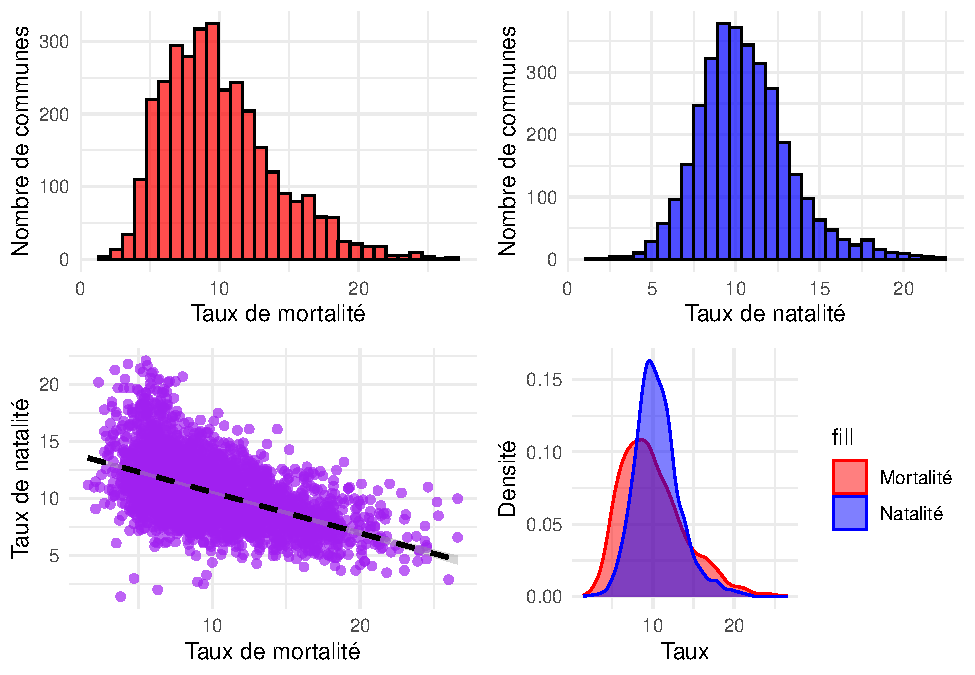
\includegraphics{Rapport_Projet_Stat_Ensai_files/figure-latex/unnamed-chunk-4-1.pdf}
Pour prendre en compte l'effet de la taille des variables et rendre les
comparaisons plus équitables, nous les avons standardisées. Aucune
catégorie ne semble montrer une relation linéaire évidente avec le taux
de visite. Par ailleurs, pour toutes les catégories
socio-professionnelles, la majorité des communes se situent dans une
plage de proportions faibles, ce qui limite la variabilité observable
dans les relations. Une analyse statistique supplémentaire, comme le
calcul de corrélations, serait nécessaire pour confirmer ou infirmer les
relations observées visuellement.

\paragraph{Analyse de corrélation}\label{analyse-de-corruxe9lation}

Les résultats de la corrélation de Pearson sont consignées dans le
tableau suivant :

\begin{longtable}[]{@{}
  >{\raggedright\arraybackslash}p{(\columnwidth - 8\tabcolsep) * \real{0.0543}}
  >{\raggedright\arraybackslash}p{(\columnwidth - 8\tabcolsep) * \real{0.5652}}
  >{\raggedleft\arraybackslash}p{(\columnwidth - 8\tabcolsep) * \real{0.1304}}
  >{\raggedleft\arraybackslash}p{(\columnwidth - 8\tabcolsep) * \real{0.1087}}
  >{\raggedright\arraybackslash}p{(\columnwidth - 8\tabcolsep) * \real{0.1413}}@{}}
\caption{Corrélations de Pearson entre le taux de consultation et les
autres variables}\tabularnewline
\toprule\noalign{}
\begin{minipage}[b]{\linewidth}\raggedright
\end{minipage} & \begin{minipage}[b]{\linewidth}\raggedright
Variable
\end{minipage} & \begin{minipage}[b]{\linewidth}\raggedleft
Correlation
\end{minipage} & \begin{minipage}[b]{\linewidth}\raggedleft
P\_value
\end{minipage} & \begin{minipage}[b]{\linewidth}\raggedright
Significatif
\end{minipage} \\
\midrule\noalign{}
\endfirsthead
\toprule\noalign{}
\begin{minipage}[b]{\linewidth}\raggedright
\end{minipage} & \begin{minipage}[b]{\linewidth}\raggedright
Variable
\end{minipage} & \begin{minipage}[b]{\linewidth}\raggedleft
Correlation
\end{minipage} & \begin{minipage}[b]{\linewidth}\raggedleft
P\_value
\end{minipage} & \begin{minipage}[b]{\linewidth}\raggedright
Significatif
\end{minipage} \\
\midrule\noalign{}
\endhead
\bottomrule\noalign{}
\endlastfoot
cor & population\_municipale\_2021\_x & 0.0765022 & 0.0000118 & Oui \\
cor1 & part\_des\_pers\_agees\_de\_75\_ans\_ou\_2021 & -0.6258560 &
0.0000000 & Oui \\
cor2 & population\_de\_15\_ans\_ou\_selon\_la\_csp\_2021\_retraites &
-0.0285517 & 0.1024362 & Non \\
cor3 & population\_de\_15\_ans\_ou\_selon\_la\_csp\_2021\_ouvriers &
0.1077559 & 0.0000000 & Oui \\
\end{longtable}

Les résultats nous montrent que le taux de consultation est positivement
corrélé à la population ainsi qu'à celle de plus de 15 ans. Cependant la
corrélation est faible. Par ailleurs, la corrélation est négative avec
la part des personnes agées de plus de 75 ans. Cela dit, plus la part
des plus de 75 ans augmente moins est le taux de consultations dans une
commune. Cela peut vouloir dire que les personnes de plus de 75 ans sont
ceux qui ne se consultent pas assez. On peut voir cela à partir de ce
graphique ci dessous.

\begin{figure}

{\centering 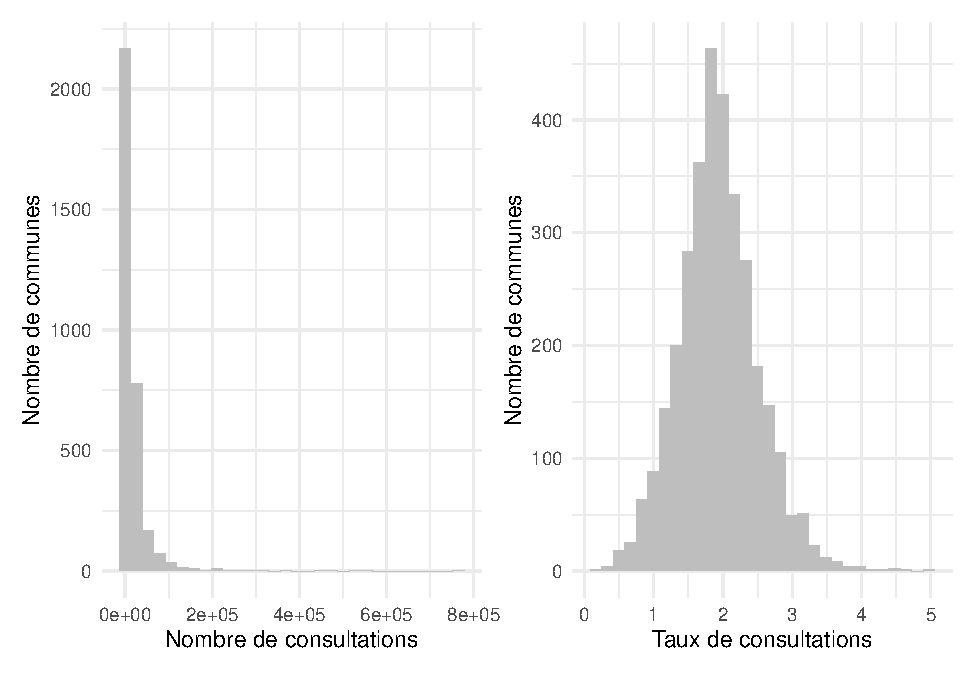
\includegraphics{Rapport_Projet_Stat_Ensai_files/figure-latex/unnamed-chunk-6-1} 

}

\caption{Relation entre taux de consultations et part des plus de 75 ans}\label{fig:unnamed-chunk-6}
\end{figure}

\subsubsection{Autocorrélation}\label{autocorruxe9lation}

L'autocorrélation spatiale est une mesure essentielle pour analyser la
dépendance entre des observations géographiques. Dans notre étude nos
données sont des données portant sur des communes. Ainsi il peut exister
une dépendance entre nos taux de consultations du fait de la proximité
des communes ou de l'appartenance à un même département ou région. Ainsi
nous allons mesurer cette dépendance en évaluant l'autocorrélation
spatiale. Dans ce contexte, \textbf{l'indice de Moran} est largement
utilisé pour quantifier cette dépendance en fournissant une mesure
globale de l'autocorrélation spatiale.

\paragraph{Définition de l'indice de
Moran}\label{duxe9finition-de-lindice-de-moran}

L'indice de Moran (\(I\)) évalue la similitude des valeurs d'une
variable entre différentes entités géographiques (par exemple, des
communes) en fonction de leur proximité spatiale. Il se base sur la
matrice de poids spatiale (\(W\)), qui définit les relations entre ces
entités.

\paragraph{Formule de l'indice de
Moran}\label{formule-de-lindice-de-moran}

La formule mathématique de l'indice de Moran est la suivante :

\[
{\raisebox{2.5em}[0pt]{\textbf{\textcolor{brown}{Formule 1}}} \hspace{5mm}
\boxed{
I = \frac{n}{\sum_{i=1}^n \sum_{j=1}^n w_{ij}} \cdot \frac{\sum_{i=1}^n \sum_{j=1}^n w_{ij} (x_i - \bar{x})(x_j - \bar{x})}{\sum_{i=1}^n (x_i - \bar{x})^2}
}
}
\]

Où : - \(n\) : Nombre total d'entités spatiales (Ici, le nombre de
communes). - \(x_i, x_j\) : Valeurs observées de la variable pour les
entités \(i\) et \(j\) (Ici le taux de consultations) - \(\bar{x}\) :
Moyenne de la variable \(x\). - \(w_{ij}\) : Poids spatial définissant
la relation entre \(i\) et \(j\).

La matrice de \(W\) peut être constuit sur la base du voisinage entre
les deux communes ou soit de la distance entre les deux communes. Dans
le premier cas alors \(w_{ij}\) \(w_{ij} = 1\) si \(i\) et \(j\) sont
voisins et \(w_{ij} = 0\) sinon. Dans le second cas \(w_{ij} = d_{ij}\).
Nous allons dans notre cas utiliser une matrice de poids basée sur la
distance, notamment celle d'Haversine.

\paragraph{Matrice de poids basée sur la distance de
Haversine}\label{matrice-de-poids-basuxe9e-sur-la-distance-de-haversine}

\subparagraph{Définition de la distance de
Haversine}\label{duxe9finition-de-la-distance-de-haversine}

La distance de Haversine est une mesure de la distance entre deux points
sur une sphère, basée sur leurs coordonnées géographiques (\(latitude\)
et \(longitude\)). Elle est particulièrement utile pour les données
géographiques projetées sur une surface sphérique, comme la Terre.

\paragraph{Formule de la distance de
Haversine}\label{formule-de-la-distance-de-haversine}

Si l'on considère deux points (\(i\)) et (\(j\)), la distance
(\(d_{ij}\)) entre ces deux points sur la surface d'une sphère de rayon
(\(r\)) est donnée par :

\[
 d_{ij} = 2r \cdot \arcsin\left(\sqrt{\sin^2\left(\frac{\phi_j - \phi_i}{2}\right) + \cos(\phi_i)\cos(\phi_j)\sin^2\left(\frac{\lambda_j - \lambda_i}{2}\right)}\right)
\]

Où : - \(r\) : Rayon de la Terre (environ 6371 km). - \(\phi_i, \phi_j\)
: Latitudes des points \(i\) et \(j\) (en radians). -
\(\lambda_i, \lambda_j\) : Longitudes des points \(i\) et \(j\) (en
radians).

\paragraph{Construction de la matrice de
poids}\label{construction-de-la-matrice-de-poids}

Pour construire la matrice de poids, nous avons alors suivi ces étapes.
*

\begin{enumerate}
\def\labelenumi{\arabic{enumi}.}
\tightlist
\item
  Calculer les distances de Haversine entre chaque paire d'entités.
\item
  Définir un seuil de distance maximale (\(d_{max}\)) :

  \begin{itemize}
  \tightlist
  \item
    Si \(d_{ij} < d_{max}\), \(w_{ij} = \frac{1}{d_{ij}}\).
  \item
    Sinon, \(w_{ij} = 0\).
  \end{itemize}
\item
  Normaliser les poids pour que chaque ligne de la matrice ait une somme
  égale à 1 : \[
   w_{ij}^{norm} = \frac{w_{ij}}{\sum_{j} w_{ij}}.
  \]
\end{enumerate}

Ainsi dans notre étude, nous avons trouvé un indice de Moran égale à

\section{Discussion}\label{discussion}

\section{Conclusion}\label{conclusion}

\section{Références
bibliographiques}\label{ruxe9fuxe9rences-bibliographiques}

\section{Annexes}\label{annexes}

\end{document}
